%Example of use of oxmathproblems latex class for problem sheets
\documentclass{oxmathproblems}
\usepackage{hyperref}
\usepackage[ngerman]{babel}
\usepackage{subfig}
%(un)comment this line to enable/disable output of any solutions in the file
%\printanswers

%define the page header/title info
\oxfordterm{14.07.2021}
\course{Vorlesung: DS-ML-PL SS21}
\sheetnumber{3}
\sheettitle{Orientierung von Äpfeln} %can leave out if no title per sheet

% add further contact details to footer if desired,
%e.g. email address, or name and email address
\contact{Juan Arango: ara@biba.uni-bremen.de, Nicolas Jathe: jat@biba.uni-bremen.de}


\begin{document}
\begin{questions}
\miquestion
Nach dem Aussortieren der schlechten Äpfel werden die verbliebenen Äpfel in Pappschalen einsortiert und mit einer Folie umwickelt. Damit die Folie nicht von den Stängeln der Äpfel durchstochen wird, müssen diese entsprechend platziert werden. Ein Roboterarm soll die automatische Platzierung übernehmen und benötigt dafür die Orientierung der Äpfel auf dem Förderband. Nutzen Sie die aus der Vorlesung bekannten Methoden um eine Regression des Winkels, der die Orientierung der Äpfel wiedergibt, durchzuführen. Nutzen Sie dafür die Bilder aus dem Datensatz \url{https://data.ips.biba.uni-bremen.de/Lehre/dsmlpl_SS21/Apples_Reg_all.tgz} und nehmen Sie an, dass ein Apfel rotationssymmetrisch ist. Der jeweilige Dateiname enthält die nötigen Informationen:
Beispiel: \texttt{0003\textunderscore X\textunderscore 045\textunderscore Z\textunderscore 06.png} ergibt die Bildnummer 3, den Winkel in $X = 45^{\circ}$ und den Winkel in $Z = 6^{\circ}$.
Im StudIP finden Sie ein Notebook, welches Sie als Grundlage nutzen können. 
\begin{parts}
  \part Unterteilen Sie die Daten selbstständig in Training- und Testdaten.
  \part Schreiben Sie eine Funktion die aus den Dateinamen die Orientierung in X extrahiert. Es könnte hilfreich sein reguläre Ausdrücke zu verwenden.
  \part Verwenden Sie die vorgefertigte Fehlerfunktion.
  \part Erstellen Sie ein eigenes Neuronales Netz oder nutzen Sie ein vorgefertigtes und trainieren Sie es so, dass es aus den Bildern die Orientierung der Äpfel als Winkel relativ zur x Achse ausgibt.
  \part Überprüfen Sie die Performance Ihrer Lösung auf den Testdaten.
\end{parts}
\begin{figure}
    \centering
    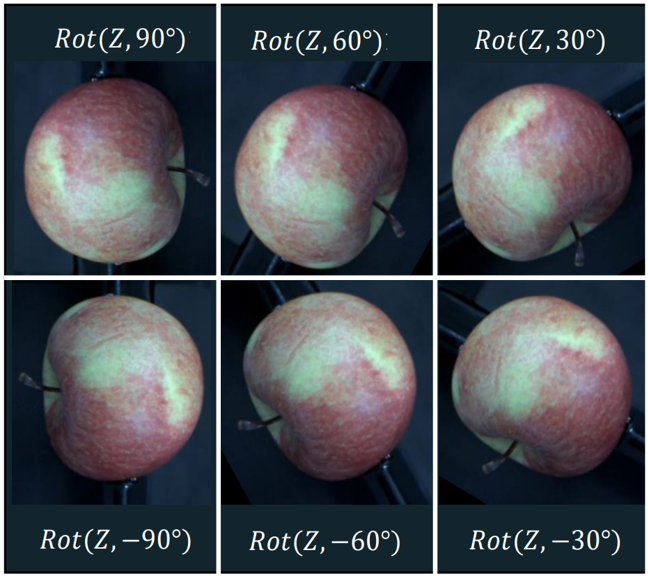
\includegraphics[scale=0.65]{rotationaepfel.png}
    \caption{Äpfel in unterschiedlichen Orientierungen.}
    \label{fig:my_label}
\end{figure}


\begin{solution}
  The solution would go here
\end{solution}
\end{questions}

\end{document}
